\subsubsection{Estados del sistema}\label{subsubsec:estados}

Los estados del sistema se controlan midiendo la tensión del panel solar y de la batería de backup con los \texttt{INA226} y cambiando los relés con el \texttt{ESP8266}. En las figuras se han omitido los componentes que no son relevantes para la explicación de los estados del sistema, es decir, los convertidores, cargadores e \texttt{INAs}. Ahora se procede a explicar cada posibe estado del sistema.

Por defecto, el sistema iniciará \textbf{alimentado por el panel solar}. En este estado, el sistema se alimenta directamente del panel solar y carga las baterías \texttt{BACKUP}, \texttt{BAT1} y \texttt{BAT2}.

\begin{figure}[H]
    \centering
    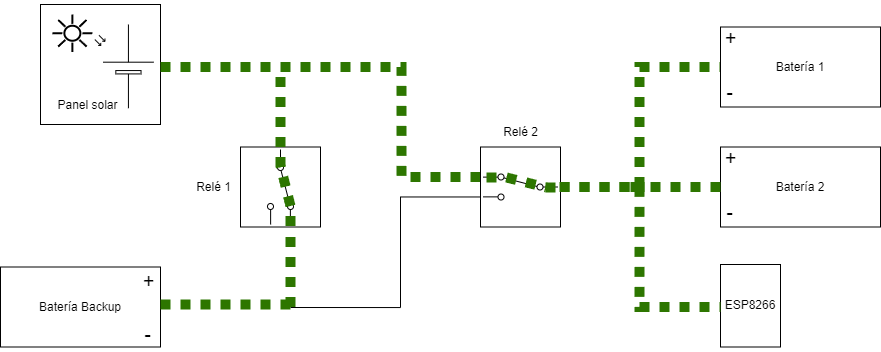
\includegraphics[width=0.7\textwidth]{images/2-hardware/Estado_solar.png}
    \caption{Sistema alimentado por el panel solar}
    \label{fig:hardware/estados/solar}
\end{figure}

En caso de que el panel solar no proporcione suficiente energía, el sistema pasará a \textbf{alimentarse de la batería de backup} gracias a los relés. En este estado, el sistema se alimenta de la batería de backup y carga las baterías \texttt{BAT1} y \texttt{BAT2}. Cuando se detecte que el panel solar vuelve a proporcionar suficiente energía, el sistema volverá al estado anterior.

\begin{figure}[H]
    \centering
    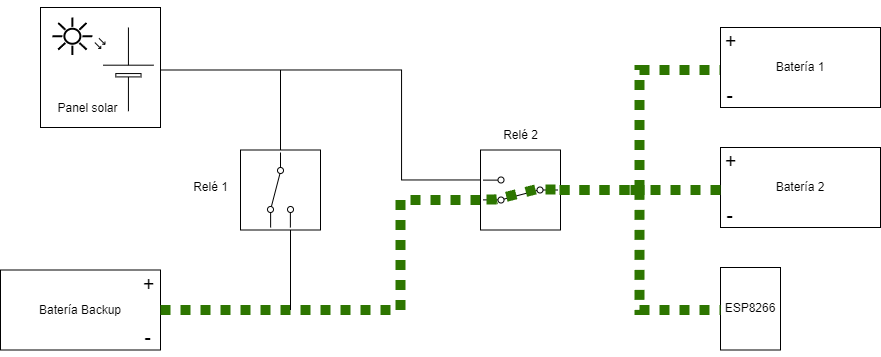
\includegraphics[width=0.7\textwidth]{images/2-hardware/Estado_backup.png}
    \caption{Sistema alimentado por la batería de backup}
    \label{fig:hardware/estados/backup}
\end{figure}

En caso de que la tensión de la batería baje por debajo del umbral establecido, el sistema pasará a su \textbf{estado por defecto}, es decir, los relés estarán configurados con el normalmente cerrado. De esta manera, el sistema se encederá automáticamente cuando el panel solar proporcione suficiente energía.

\begin{figure}[H]
    \centering
    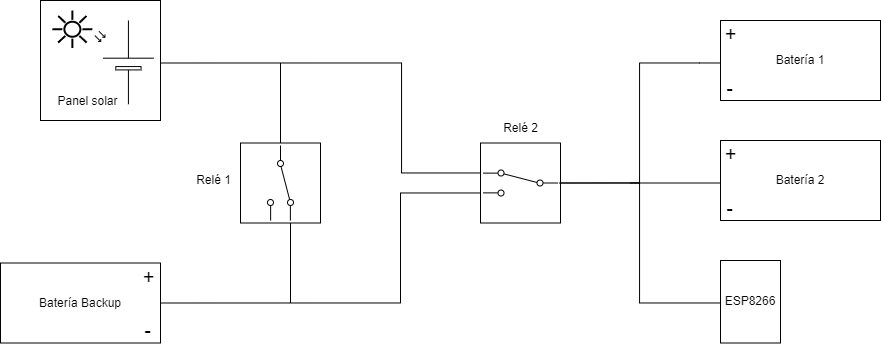
\includegraphics[width=0.7\textwidth]{images/2-hardware/Estado_defecto.png}
    \caption{Estado por defecto}
    \label{fig:hardware/estados/defecto}
\end{figure}
